
\documentclass[border=4pt]{standalone}
\usepackage[utf8]{inputenc}
\usepackage[T1]{fontenc}
\usepackage{amsmath,amssymb,xcolor}
\usepackage{tikz}
\usetikzlibrary{arrows.meta,shapes.misc}
\renewcommand{\familydefault}{\sfdefault}
\definecolor{vbleu}{HTML}{1C5FD6}
\definecolor{orange}{HTML}{E8590C}
\definecolor{vert}{HTML}{2F9E44}
\definecolor{gris}{HTML}{495057}
\definecolor{violet}{HTML}{7048E8}
\tikzset{
  vec/.style={->,very thick,>={Stealth[length=2.4mm]}},
  ref/.style={orange,thick,dashed},
  par/.style={vert,thick,dashed},
  sec/.style={gris,thick,dashed},
  ptcross/.style={cross out,draw,thick,minimum size=1.6mm,inner sep=0pt},
}
\usepackage{array}
\setlength{\parindent}{0pt}\setlength{\parskip}{5pt}
\newcommand{\V}[1]{\overrightarrow{\mathrm{#1}}}
\begin{document}

\begin{minipage}{16cm}\large {\color{vert}\Large Étape 1 — On repère la direction de $\vec{t}$}\par\vspace{4pt}{\centering 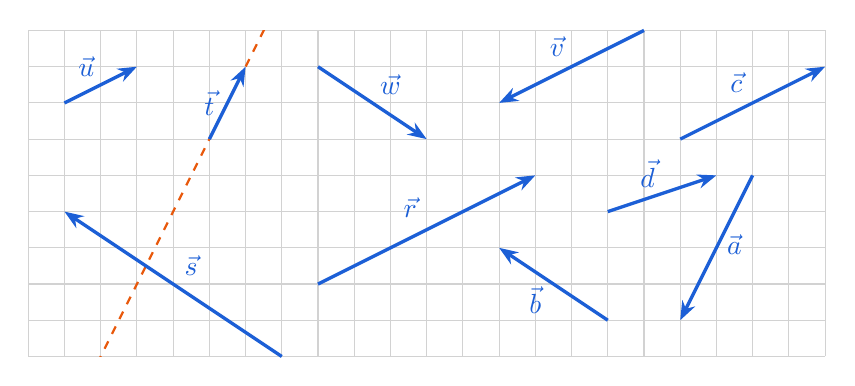
\begin{tikzpicture}[x=0.46cm,y=0.46cm]
\draw[gray!35,thin,step=0.46cm] (0,0) grid (22,9);
\begin{scope}\clip (0,0) rectangle (22,9);
\draw[ref] (-35,-74) -- (45,86);
\end{scope}
\draw[vec,vbleu] (1,7) -- (3,8);
\node[vbleu] at (1.6,8.0) {$\vec{u}$};
\draw[vec,vbleu] (5,6) -- (6,8);
\node[vbleu] at (5.0,7.0) {$\vec{t}$};
\draw[vec,vbleu] (8,8) -- (11,6);
\node[vbleu] at (10.0,7.5) {$\vec{w}$};
\draw[vec,vbleu] (17,9) -- (13,7);
\node[vbleu] at (14.6,8.55) {$\vec{v}$};
\draw[vec,vbleu] (18,6) -- (22,8);
\node[vbleu] at (19.55,7.55) {$\vec{c}$};
\draw[vec,vbleu] (20,5) -- (18,1);
\node[vbleu] at (19.5,3.1) {$\vec{a}$};
\draw[vec,vbleu] (16,1) -- (13,3);
\node[vbleu] at (14.0,1.55) {$\vec{b}$};
\draw[vec,vbleu] (16,4) -- (19,5);
\node[vbleu] at (17.1,5.05) {$\vec{d}$};
\draw[vec,vbleu] (7,0) -- (1,4);
\node[vbleu] at (4.5,2.5) {$\vec{s}$};
\draw[vec,vbleu] (8,2) -- (14,5);
\node[vbleu] at (10.55,4.1) {$\vec{r}$};
\end{tikzpicture}\par}\vspace{4pt}On trace la droite qui porte le vecteur $\vec{t}$ (en pointillés orange).\end{minipage}
\end{document}
